\documentclass[a4paper,12pt]{article}
\usepackage[utf8]{inputenc}
\usepackage{amssymb,amsmath,uniinput,graphicx,hyperref, multirow,siunitx}
\usepackage[section]{placeins}
\usepackage[ngerman]{babel}
\usepackage[left=3cm,right=3cm,top=3cm,bottom=3cm]{geometry}
\renewcommand{\familydefault}{\sfdefault}
\setlength{\belowcaptionskip}{6pt}
\hypersetup{pdfinfo = {
	Title={Versuchsprotokoll zu Positronen im Festkörper},
	Author={Knut Kiesel, Tobias Pook},
	Keywords={Teilchenfalle}
}}


\graphicspath{ {../pictures/} }
\title{Laborpraktikum Teilchenphysik\\ Lebensdauer von Positronen im Festkörper}
\author{Knut Kiesel\\Tobias Pook}
\date{\today}

\begin{document}
\maketitle
\vspace{5cm}
\tableofcontents
\thispagestyle{empty}
\newpage
\setcounter{page}{1}

\section{Ziel des Versuches}
Ziel des Versuches ist der Aufbau und die Inbetriebnahme einer Messstation,
die in der Lage ist die Lebensdauer von Positronen in Festkörpern in der
Größenordnung von $\si{ps}$ zu messen.

Hierzu wird $^{22}$Na verwendet, welches beim Zerfall in $^{22}$Ne
zuerst ein γ-Quant der Energie $1.28\si{MeV}$ abgibt und dann ein Positron emittiert.
Nach einer vom Festkörper abhängigen Zeit annihiliert das Positron unter Aussendung
von 2 bis 3 γ Quanten der Energie von $0.511\si{keV}$.
Durch das messen der Zeitdifferenz zwischen dem ersten γ-Quant des Übergangs zum
Annihilierquant kann die Lebensdauer des Positrons bestimmt werden.




\section{Aufbau und Durchführung}

\begin{figure}[htb]
		\centering
		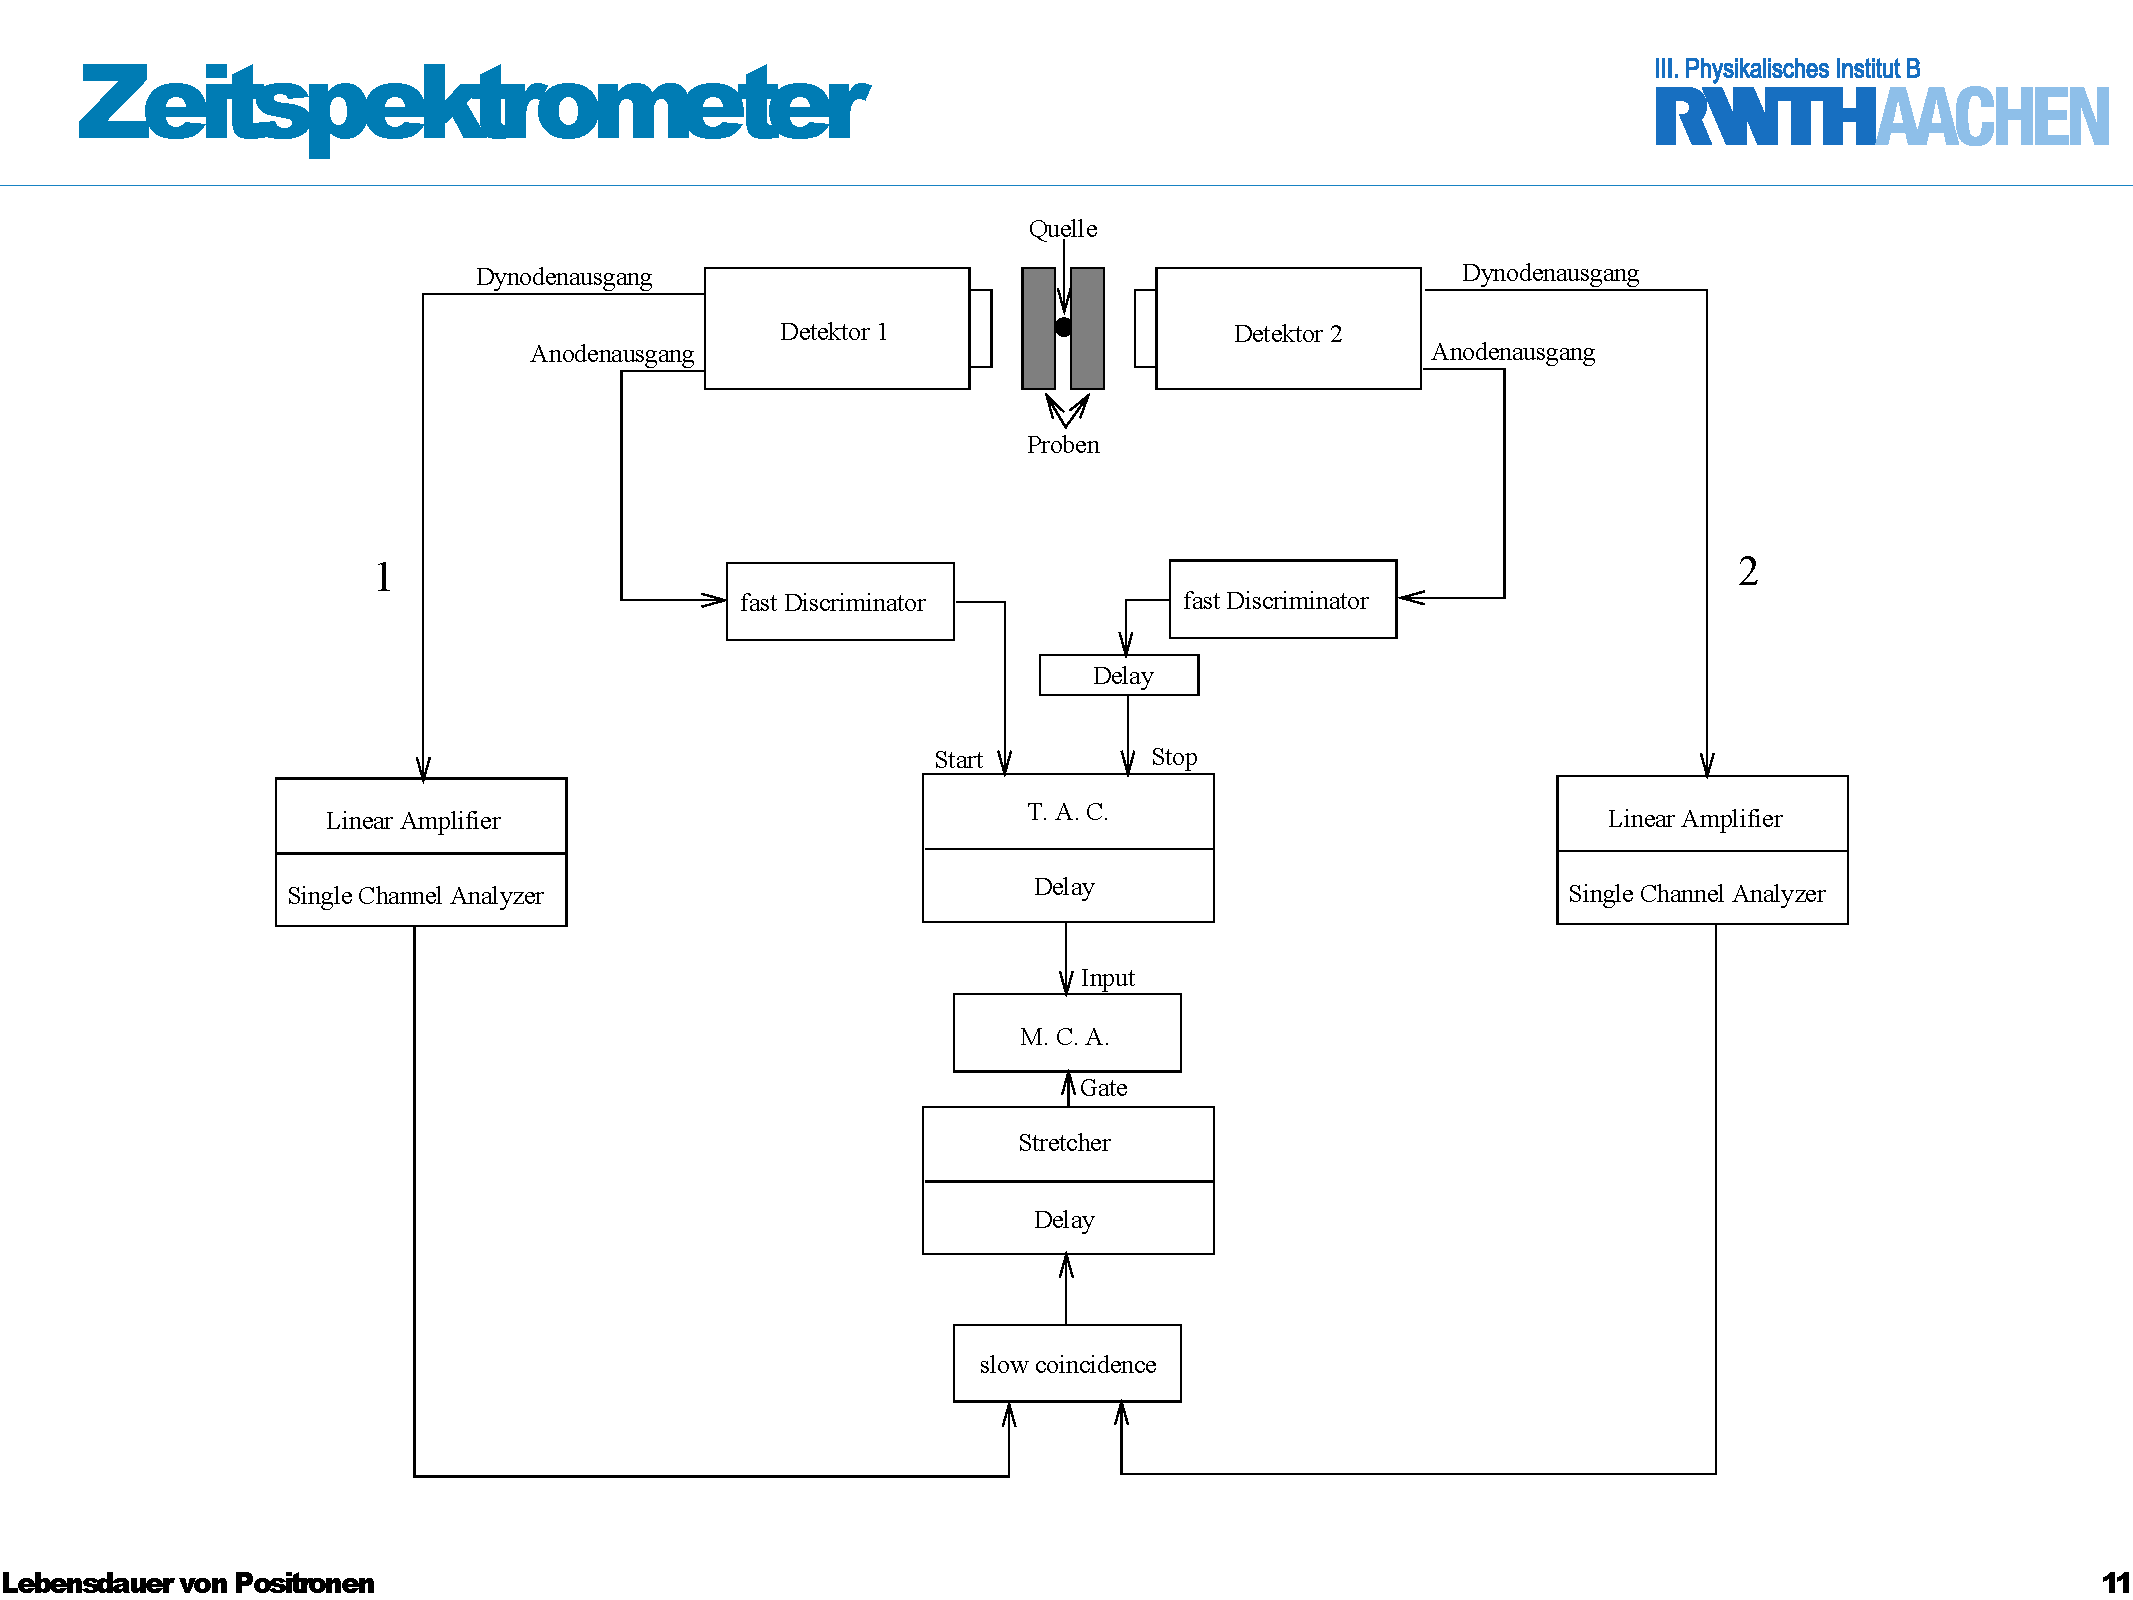
\includegraphics[width=0.8\textwidth]{schaltplan.pdf}
		\caption{Schaltplan}
		\label{fig:schaltplan}
\end{figure}
\section{Ergebnisse}

\section{Diskussion}
\end{document}
